\chapter{Simulation}
Die Simulationen werden vom Grundaufbau wie folgt umgesetzt, sie bestehen aus einem Konfigurationsskript, welches die Parameter für das eigentliche Modell in den Matlab Workspace lädt und die Automatisierung der Simulationsdurchläufe umsetzt. Das Modell wird in Simulink über PLECS Blockset aufgebaut und durch einen Output als gebündelte Schnittstelle werden die Daten an Matlab zurückgeführt. Die Rückführung der Daten wird für die Simulationen einheitlich in festgelegter Reihenfolge zusammengeführt, siehe Abb. 

\begin{figure}
	\centering
	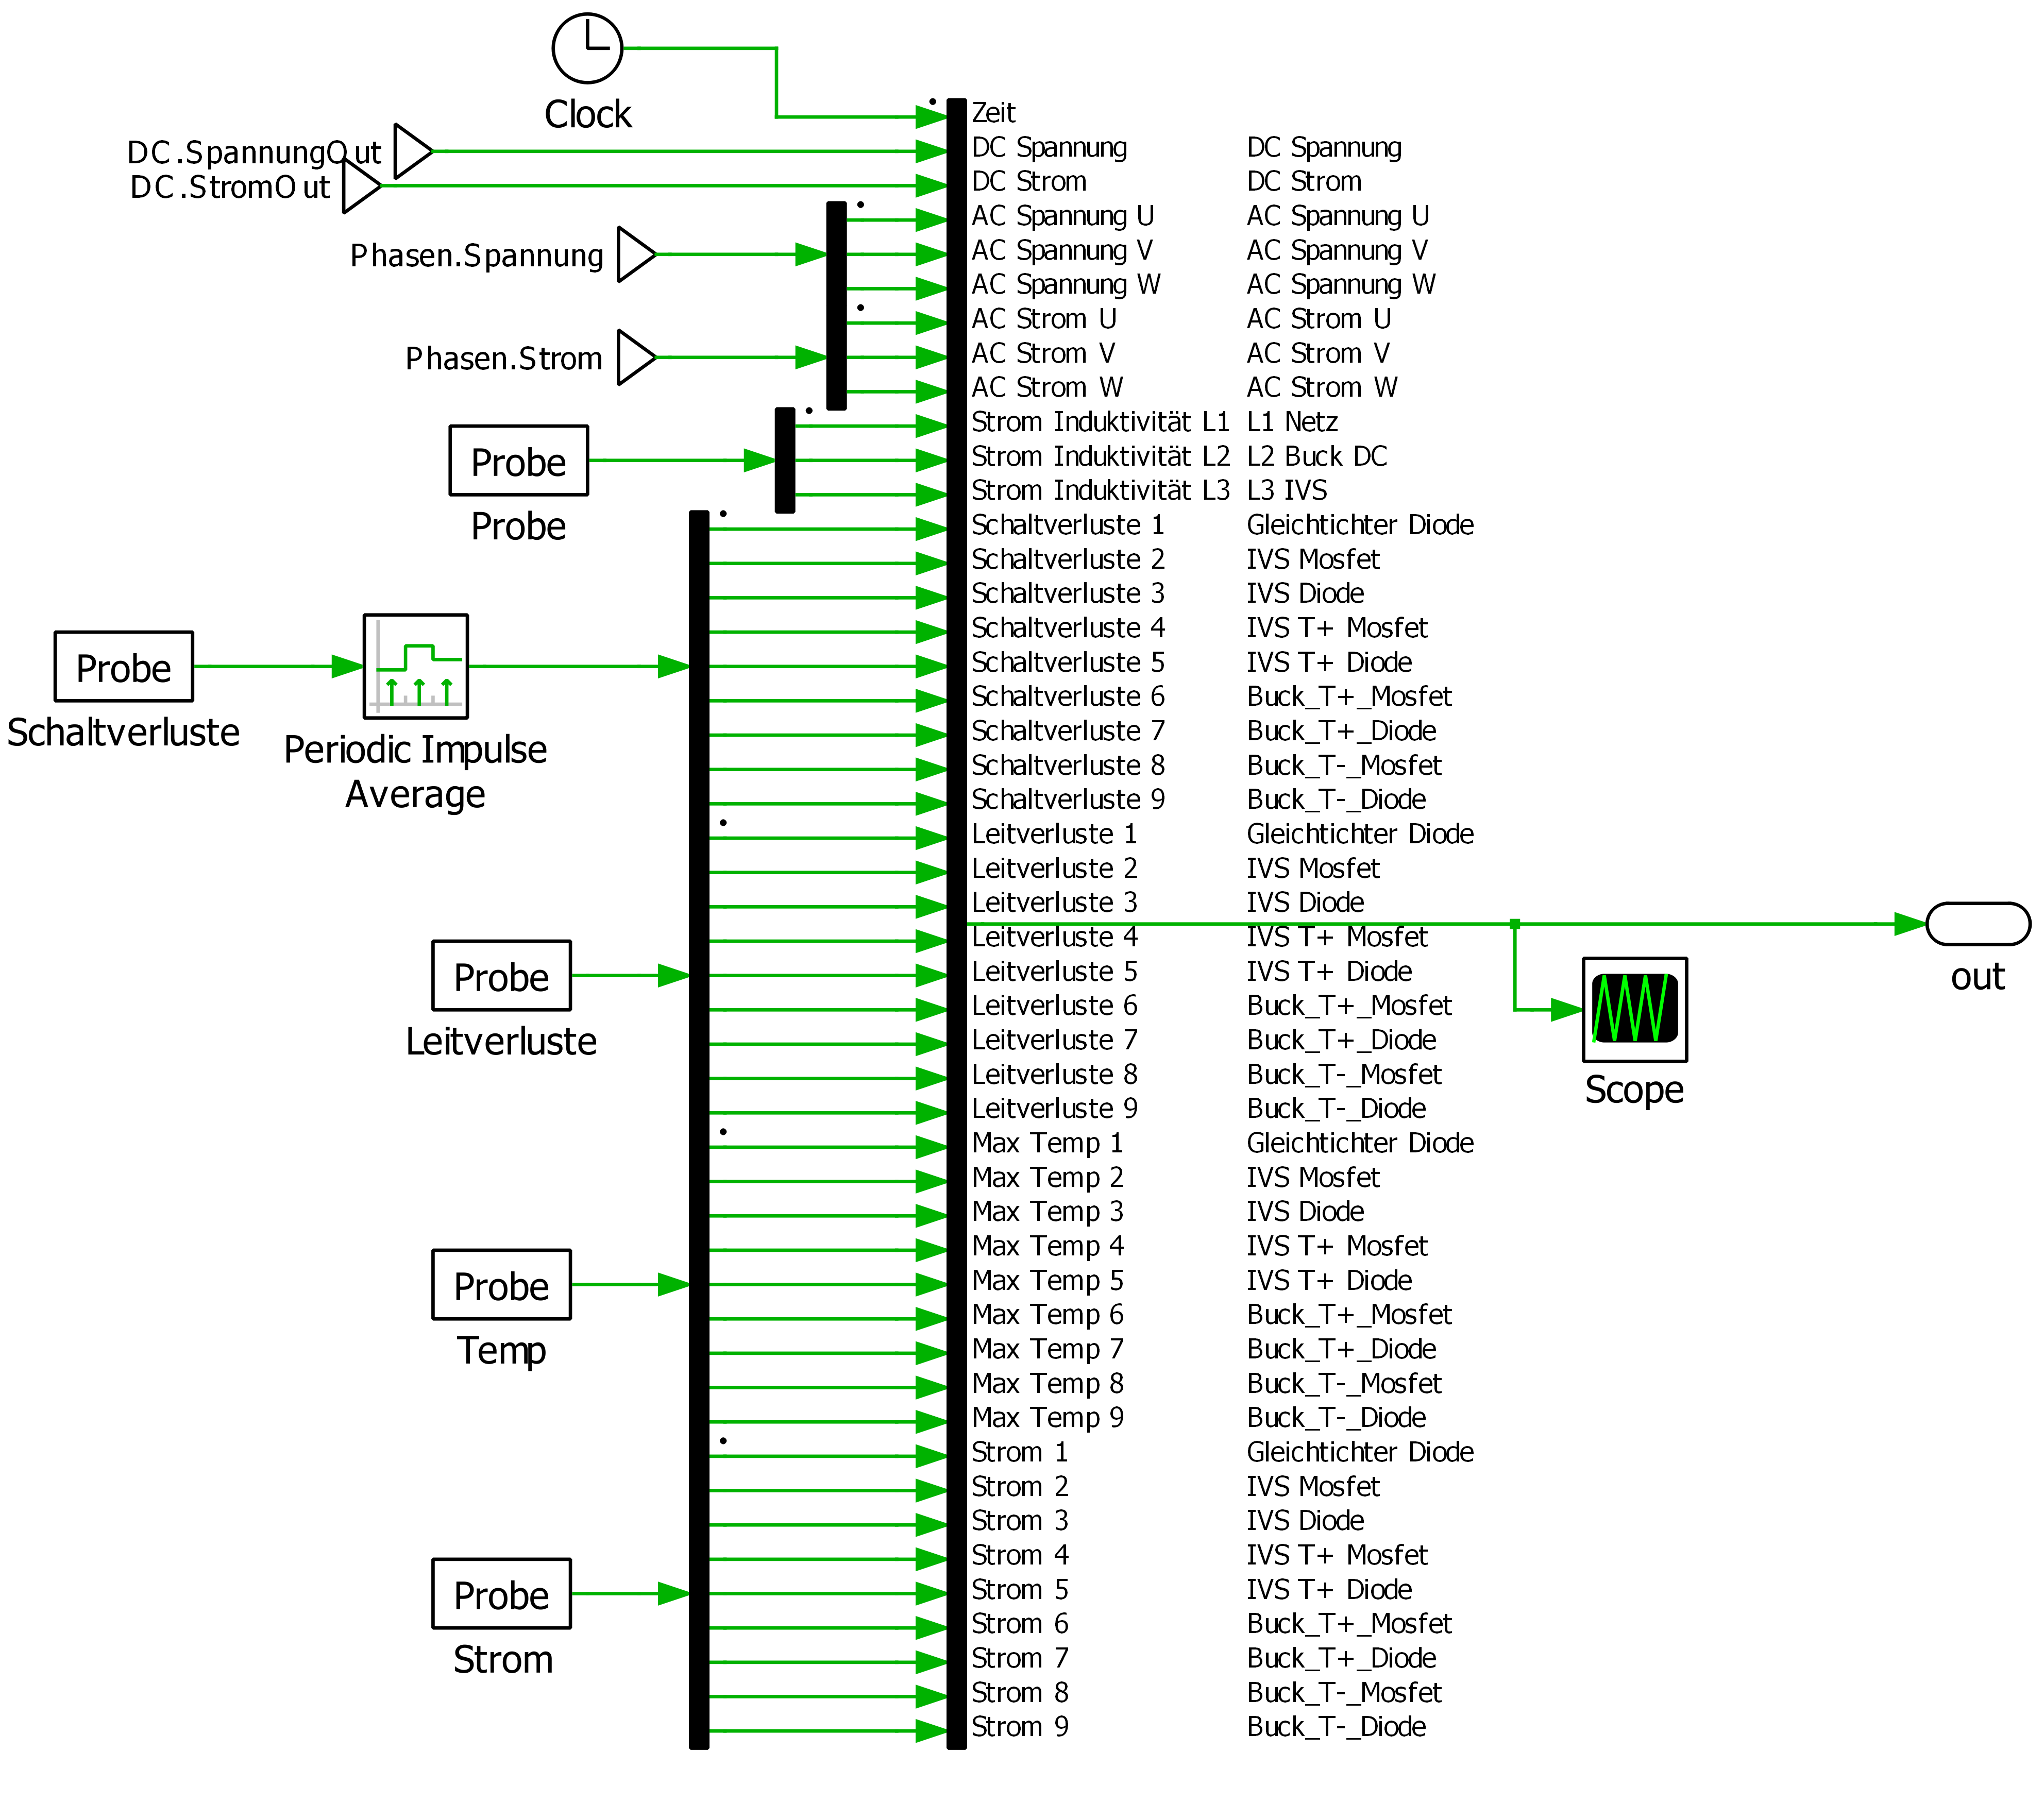
\includegraphics[width=0.7\linewidth]{content/Grafiken/Plecs_Out}
	\caption[Zusammenfassung der Simulationsoutputs]{Zusammenfassung der Simulationsoutputs}
	\label{fig:plecsout}
\end{figure}

\section{Randbedingungen}
Für den Gleichrichter werden Grundlegende Parameter festgelegt um die Auslegung für die Simulation durchführen zu können. 

\begin{itemize}
	\item Ausgangsleistung: 200 kW
	\item Ausgangsspannung: 482-680 V
	\item Ausgangsstrom: 	295 A
	\item \gls{Ull}:		617 V
	\item Netzfrequenz		50 Hz
	\item Filterblindleistung: 3 \%
	\item Schaltfrequenz: 20 kHz
	\item Netzspannungsschwankung: 10%
\end{itemize}

Die Regelung benötigt eine Erkennung des aktuellen Phasenwinkelabschnitts, diese ist implementiert nach \cite{InstituteofElectricalandElectronicsEngineers}.

\section{Tiefsetzsteller}

	\subsection{Auslegung der Induktivität}
	Die Speicherdrossel wird anhand von Formel \ref{eq:BuckL} ausgelegt, dabei liegt die Netzspannung bei maximal $ U_{LLmaxPeak}=1,1 \cdot 617 \si{\V} \cdot \sqrt{2}=959,8 \si{\V} $ und die Ausgangsspannung bei mindestens 482 \si{\V}. Daraus ergeben sich die maximalen Parameter, die der Tiefsetzsteller umsetzen muss. Es ergibt sich somit eine Induktivität von 134,16 \si{\micro \henry}, siehe Formel \ref{eq:BuckLwert}.
	 \begin{equation}
	 	\label{eq:BuckLwert}
	 	L_{T}=\dfrac{959,8\si{\V} - 482 \si{\V}}{20 \si{\kilo \hertz}\cdot 0,3 \cdot 295 \si{\ampere}}\cdot \dfrac{482 \si{\V}}{969,8 \si{\V}}= 134,16 \si{\micro \henry} 
	 \end{equation}

\section{IAF}

	\cite{IAF99}
	
	\subsection{Auslegung der Induktivität}
	Der maximale Stromrippel ergibt sich aus der Leistung und der minimalen Netzspannung und beträgt 44,1 \si{\A}, siehe Formel \ref{eq:DeltaIIVS}.
	
	\begin{equation}
		\label{eq:DeltaIIVS}
		I_{\Delta max IVS}= \dfrac{0,3\cdot \sqrt{2} \cdot 200 \si{\kilo \watt}}{2 \cdot \sqrt{3} \cdot 617 \si{V} \cdot 0,9 = 44,1 \si{\A}}
	\end{equation}
	
	\subsection{Regelung}
	
	\subsection{Ergebnisse}
	

\section{B6 1/3 PFC Buck}
Die in Kapitel \ref{sec:GrundlagenB6} dargestellte Schaltung wird durch Halbbrücken Module des Typs FF2MR12W3M1H\_B11 von Infineon implementiert. Dabei handelt es sich um verbreitete 1200 \si{\volt} Module, sie besitzen einen nominellen Einschaltwiderstand von etwa 2 \si{\milli \ohm} und können Spitzenströme von bis zu 800 \si{\ampere} schalten \cite{IFAGFF2}. Um die Ausgangsleistung auch bei geringerer Spannung bereitstellen zu können und ein späteres Interleaving zu ermöglichen werden für den Tiefsetzsteller zwei Halbbrücken vorgesehen.

	\subsection{Auslegung der Induktivität}
	
	
	\subsection{Regelung}
	Die Regelung besteht aus einer Kaskadierten Struktur mit vier Stufen. Die erste ist die Ausgangsspannungsregelung, welche durch die Sollleistung und Netzspannung die gewünschte äquivalente Phasenimpedanz als Eingangsgröße für die Phasenstromregelung bildet.\\
	In der dritten Stufe wird die Phase mit der mittleren Spannung ausgewählt und die Zwischenkreisspannung \gls{Upn} anhand der Phasenlage bestimmt. Die Zwischenkreisspannung resultiert als sechspulsige Gleichspannung und dient als Eingangsspannung für den Tiefsetzsteller. Die mittlere Phasenspannung wird als Referenz für den Tastgrad der entsprechenden Halbbrücke verwendet und prägt somit einen zur Spannung proportionalen Strom ein. Somit wird immer nur eine der drei Halbbrücken getaktet geschaltet, die anderen beiden sind wie bei einem Diodengleichrichter auf die jeweils positivste und negativste Spannung geschaltet.\\
	Die vierte Stufe ist die des Tiefsetzstellers, mit Reglern für den Eingangsstrom sowie die Ausgangsspannung.
	
	\begin{figure}
		\centering
		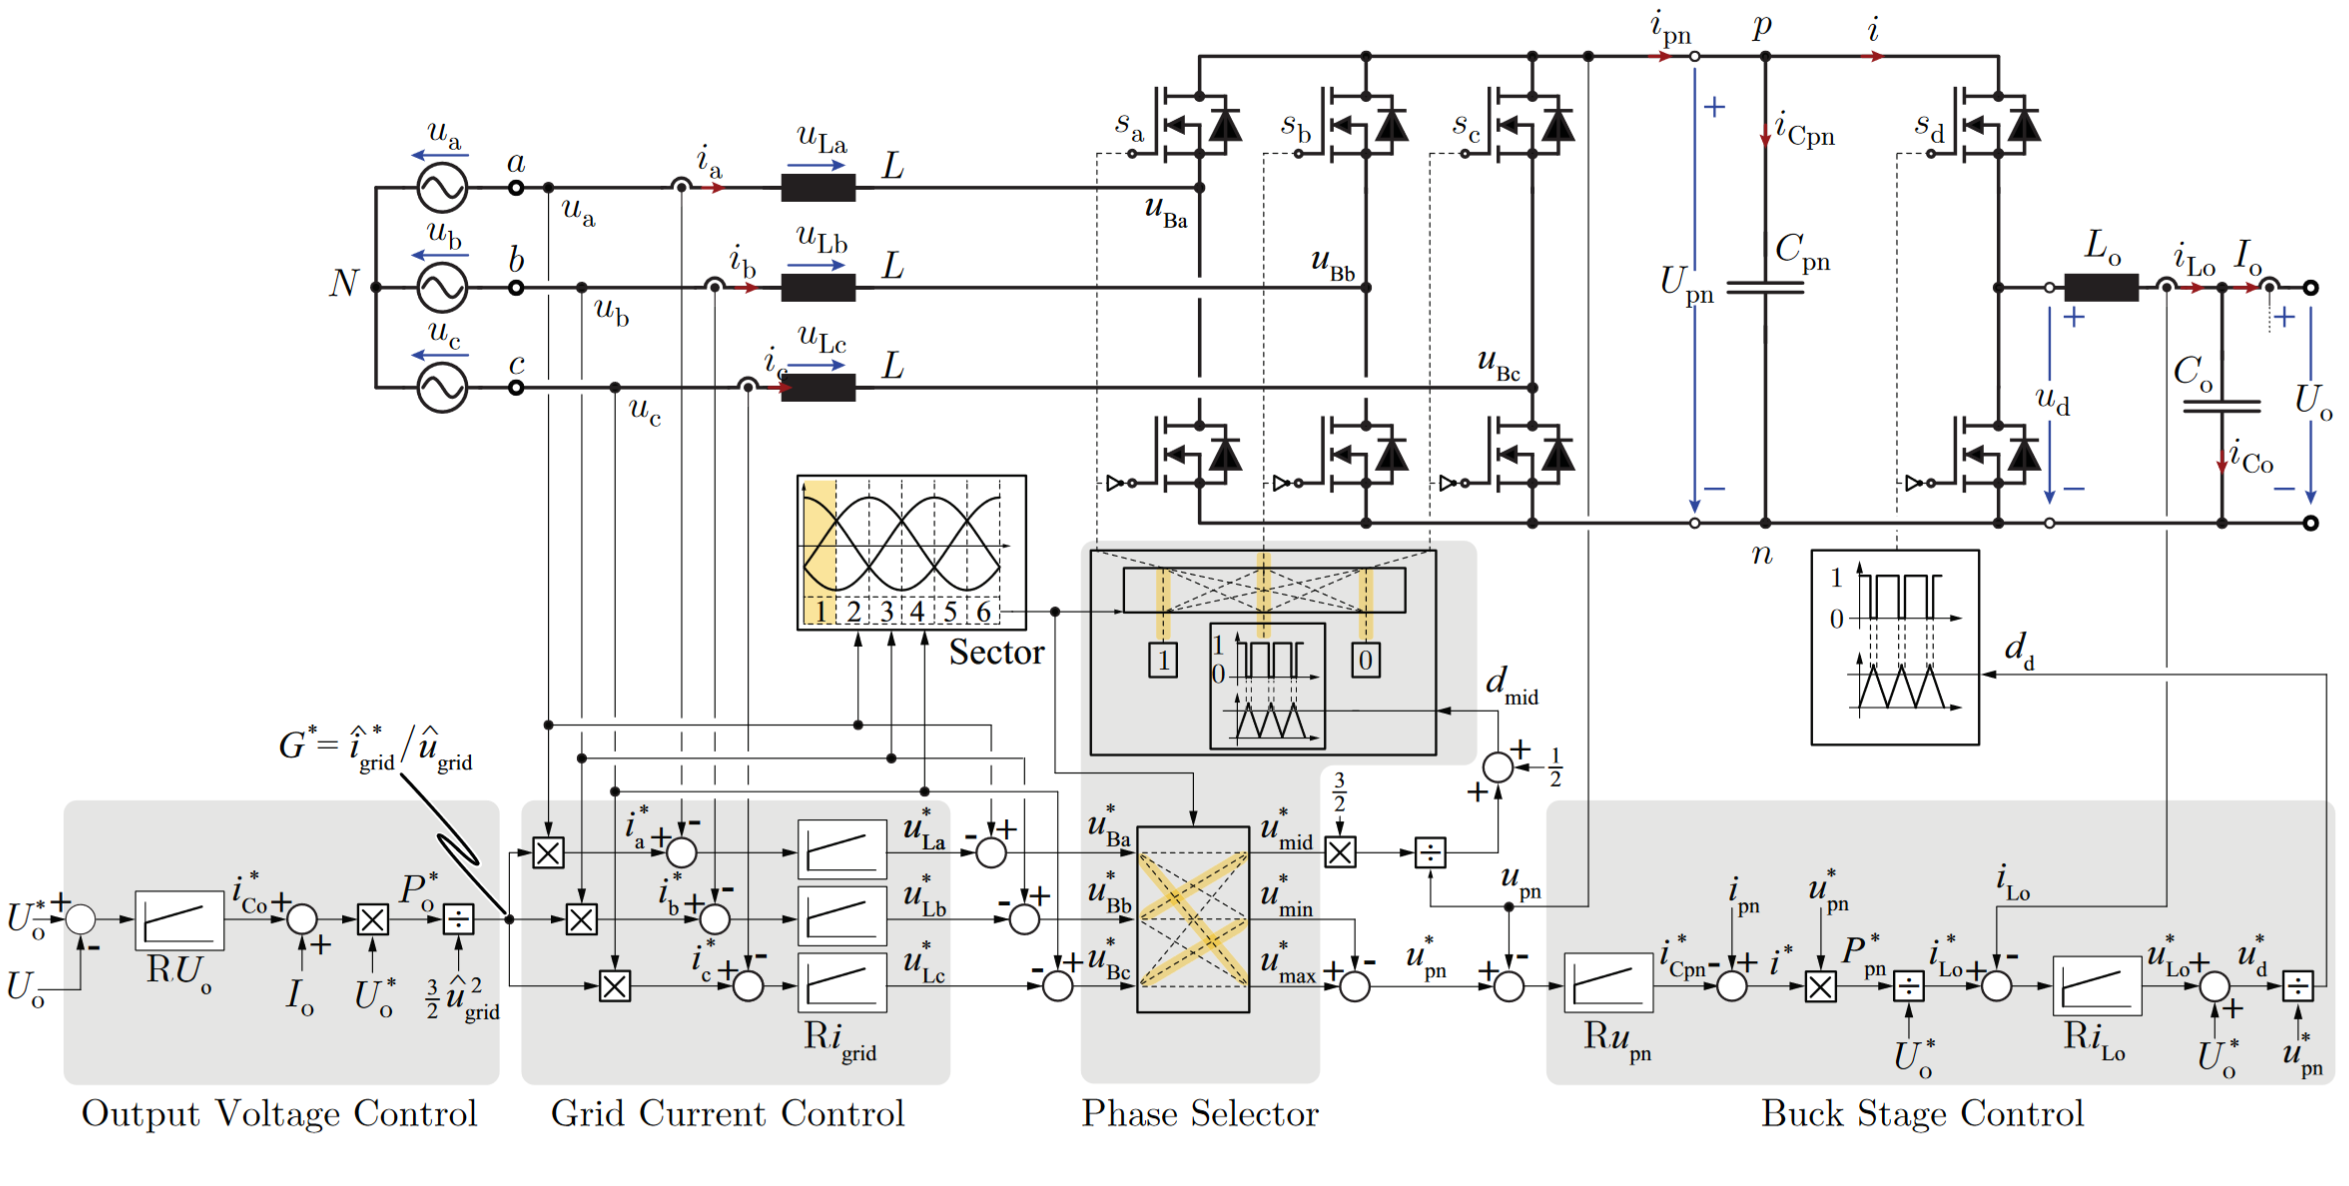
\includegraphics[width=0.9\linewidth]{content/Grafiken/B6-Control-orig}
		\caption[Regelung des \gls{B6PFC}]{Regelung des \gls{B6PFC} \cite{13PWMPFC}}
		\label{fig:b6-control-orig}
	\end{figure}
